%!TeX root=../main.tex

% TODO: Edit caption waaay down

\begin{figure}[!htb]        
\vskip -0.10in % useful knobs to optimize layout
    \centering        
    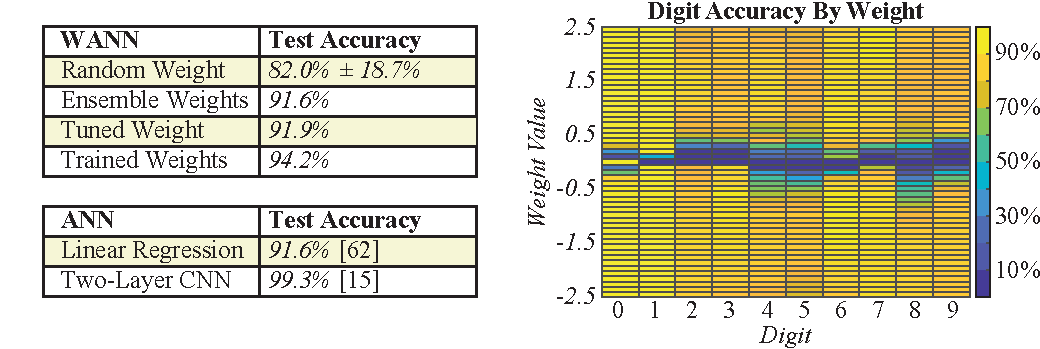
\includegraphics[width=1\textwidth]{img/mnist.pdf}   
\vskip -0.20in % useful knobs to optimize layout (going a bit overboard here, since caption is only on left side)
    \caption      
    {     
        \textit{Classification Accuracy on MNIST.
        }
        \newline
        \textit{Left:}
        WANNs instantiated with multiple weight values acting as an ensemble perform far better than when weights are sampled at random, and as well as a linear classifier with thousands of weights. 
        %
        %The accuracy of the best single weight value exceeds this. 
        \newline
        \textit{Right:} No single weight value has better accuracy on all digits. That WANNs can be instantiated as several \textit{different} networks has intriguing possibilities for the creation of ensembles.       
    }
    \label{fig:mnist}
\vskip -0.05in % useful knobs to optimize layout
\end{figure}
